\documentclass{report}
\usepackage{graphicx}
\usepackage{setspace}
\usepackage[margins=1in]{geometry}
\usepackage{color}
\usepackage{hyperref}
\usepackage{listings}

\linespread{1.5}

\lstdefinelanguage{SQL}{
	keywords = {,SELECT ,FROM,JOIN,ON,WHERE, GROUP BY, AS, AND, OR, BETWEEN, UPDATE, SET, INTO,INSERT,insert,}
	sensitive=false,
	keywordstyle = \color{blue},
	ndkeywords={OC3_comm, OC3_staff, OC3_notes, OC3_contact, OC3_contract, OC3_turningform, OC3_item},
	ndkeywordstyle = \color{red}\bfseries,
	stringstyle = \ttfamily
}
\lstset{
	language = SQL,
	extendedchars = true,
	basicstyle = \ttfamily,
	numbers = left,
	frame = leftline
	}
\begin{document}

\title{\bfseries UT Business Contracts Application Documentation}

\author{
	Coling Murray (Team Leader)
	\and
	Calvin Aisenbrey
	\and
	Alex Landaverde
	\and
	Chris Metcalf
	\and
	Ashley Ng
}

\maketitle

\begin{abstract}
Put abstract here
\end{abstract}

\tableofcontents

\newpage

\begin{image}
\centering
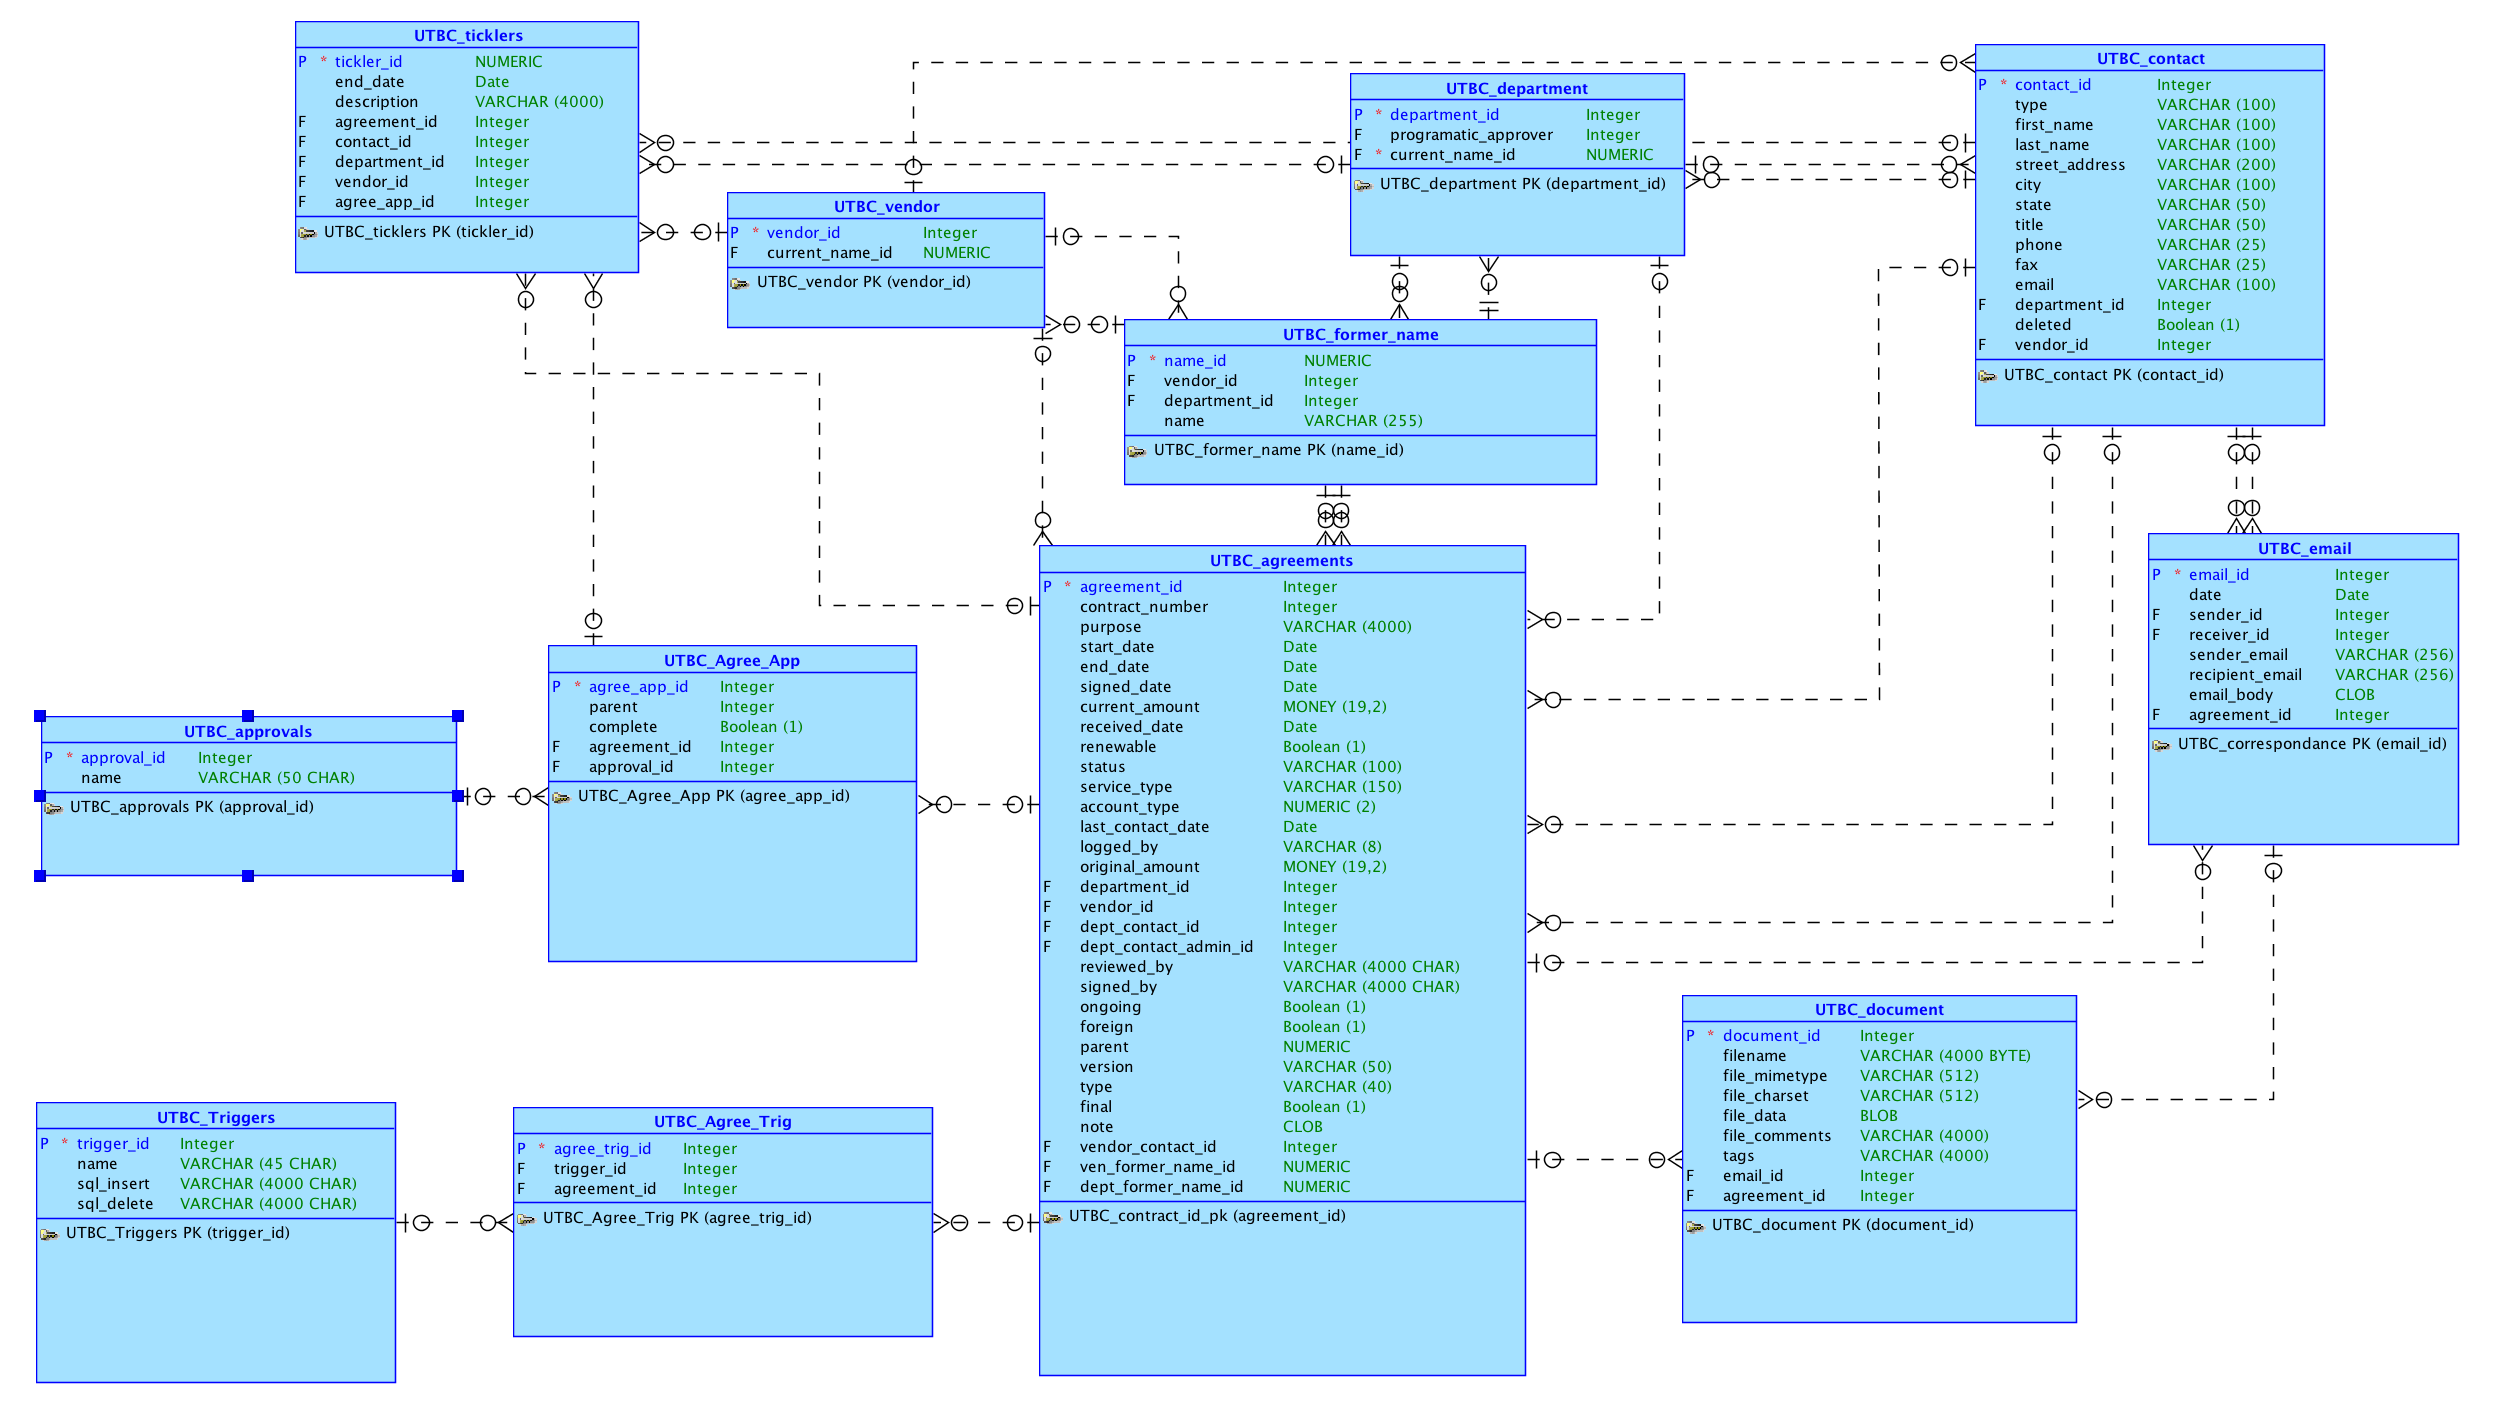
\includegraphics[height = 4.5in, angle = 90]{UTBC_model}
\end{image}



\chapter{Data model}

\section{Contract Table}

\section{UTBC\_approvals and UTBC\_Agree\_App Tables}

\section{UTBC\_triggers and UTBC\_Agree\_Trig Tables}

\chapter{Application}

\section{Home Page}
The home page consists of three different tables; contracts, ticklers, and BOR dates. The tables only displays contracts that are renewable and are expiring in the next 60 days. The table also only displays contracts that pertain to the user logged in using the where clause

\begin{lstlisting}[caption=Contracts table where clause for user]
WHERE reviewed_by APEX_UTIL.GET_SESSION_STATE('APP_USER')
\end{lstlisting}

The next table is ticklers (or reminders), which only displays ticklers pertaining to the user that is logged in as well as public ticklers for everyone to see. We used the following where clause to do this

\begin{lstlisting}[caption=Tickler table where clause]
WHERE t.created_by = APEX_UTIL.GET_SESSION_STATE('APP_USER')
OR PUBLIC_T = 'Y'
\end{lstlisting}

In this ticklers table, two tables are joined; the UTBC\_ticklers and UTBC\_contact tables. That way the user can easily email the corresponding person about the tickler. 
The next table is BOR dates (or board of regents dates). This table has no connect do our data model and is a stand alone table. The table has two attributes, due date and meeting date. The due date is the day the office will have to get certain paperwork submitted to be on the associated meeting date.

\section{Agreements Home Page}

\subsection{Agreements Tree}

\subsection{Agreements Search Bar}

\subsection{Agreements Sorting}

\subsection{Agreements Form}

\section{Agreements Details Page}

\subsection{Purpose region}

\subsection{Related Region}

\subsection{Notes Region}

\subsection{Add Sub-Agreement, Add Version}

\subsection{Approvals Region}

\section{Other Forms}

\subsection{Vendor Form}

\subsection{Department Form}

\subsection{Tickler Form}

\subsection{Document Form}
The documents form uses a file drop plug-in that was downloaded at apex-plugin.com, and was created by Damien Antipa. The file drop plugin automatically does an insert into the table (as seen from the following code) once you drop the file into the file drop window. This causes an issue for the user because they have yet to finished completing the document form, or if the user uploaded the incorrect document, or decides to cancel the form. To get around this, the document\_id was returned in the PL/SQL statement after the insert

\begin{lstlisting}[caption = PL/SQL on filedrop item]
DECLARE
  c_collection_name constant varchar2(200):='CLOB_CONTENT';
  l_blob				     BLOB;
  l_mime				     varchar2(50);
BEGIN
  SELECT apex_web_service.clobbase642blob(
  	substr(clob001, ',')+1, length(clob001)))
  INTO l_blob
  from apex_collections
  where collection_name = c_collection_name
  
  insert into UTBC_document(FILE_DATA, filename, 
  	file_mimetype, AGREEMENT_ID) 
  values(l_blob, wwv_flow.g_x01, wwv_flow.g_x02, :P28_agreement_id)
  returning document_id into :P28_document_id;
END;
\end{lstlisting}

If the user now decided that they want to cancel the form, a dynamic action fires when the user clicks the cancel button, and executes PL/SQL code

\begin{lstlisting}[caption=close dialog PL/SQL]
BEGIN
delete from UTBC_document where document_id = :P28_document_id;
END;
\end{lstlisting}

Because the file browse and file drop both have different ways of inserting the blob into the table, two different create buttons were made. One handling the file browse and another handling the file drop, but only one is ever displayed at a time because of a IS NOT NULL or IS NULL condition on the item P28\_FILENAME\_SHOW. The item is initially null, and then will be filled with the text ``*filename* uploaded" once the file drop has done the insert. 
One of the create buttons is the original create button that handles the file browse option. The other create button for the file drop option has PL/SQL code that fires when the corresponding create button is clicked. 

\begin{lstlisting}[caption=update statement for filedrop]
BEGIN
	update UTBC_document
	SEt
	file_comments = :P28_file_comments, 
	tags = :P28_tags,
	where document_id = :P28_document_id;
END;
\end{lstlisting}

At this point there is no indication when a file is successfully uploaded/inserted with the file drop. The was handled using a dynamic action event that came with the plug-in, upload ended.  To do this, a dynamic action was created on the upload ended event on the file drop item. A false action was created to fire on page load, to hide the P28\_FILENAME\_SHOW item. Next, several true actions were set up, the first being to hide the file drop window. The next was to set this P28\_FILENAME\_SHOW with the filename. A cancel upload button will also be shown after upload. This button is incase the user has accidentally selected the incorrect file. When the button is clicked, a dynamic action fires that will delete the corresponding file, show the file drop region again, and then set the P28\_FILENAME\_SHOW item back to null.
\end{document}